\chapter{Типы уравнений первого порядка}

\begin{enumerate}
	\item[\rom1.] Уравение с разделёнными переменными:
    $$ \frac{\di x}{g(x)} + \frac{\di y}{h(y)} = 0 $$
    $$ U(x, y) = \ufint{g(x)} + \ufint[y]{h(y)} + C $$
    \item[\rom2.] Уравнение с разделяющимися переменными:
    $$ g_1(x)h_2(y)\di x + g_2(x)h_1(y)\di y = 0 $$
    \antlersimp
    \begin{multicols}{2}
        $$ \frac{g_1(x)}{g_2(x)}\di x + \frac{h_1(y)}{h_2(y)}\di y = 0 $$
        \columnbreak
        $$ \left[
        \begin{aligned}
        	g_2(x) = 0 \\
            h_2(y) = 0
        \end{aligned} \right. $$
        Это всё решается (т. к. $ \di x $ и $ g_2(x) $ одновременно обратятся в 0)
    \end{multicols}
    \item[\rom3.] Линейное уравнение:
    $$ y' + p(x)y = \underset{\text{неоднородность}}{q(x)}, \qquad p(x), q(x) \in \Cont{\braket{a, b}} $$
    \begin{itemize}
    	\item Если $ q(x) \equiv 0 $, то уравнение $ y' + p(x)y = 0 $ называется линейным однородным (ЛОУ)
        \item Иначе $ y' + p(x)y = q(x) $ -- линейным неоднородным (ЛНУ)
    \end{itemize}
    $$ \underset{
        \begin{subarray}c
            \text{общее неоднородное} \\
            \text{(все реш. ЛНУ)}
        \end{subarray}}{y_{\text{ОН}}(x, C)} = \underset{
        \begin{subarray}c
            \text{общее однор.} \\
            \text{(все реш. ЛОУ)}
        \end{subarray}}{y_{\text{ОО}}(x, C)} + \underset{
        \begin{subarray}c
            \text{частное неоднор.} \\
            \text{(какое-то решение ЛНУ)}
        \end{subarray}}{y_{\text{ЧН}}(x, C)} $$
    \begin{algo}[решения]
        \item Ищем $ y_{\text{ОО}} $:
        $$ y_{\text{ОО}} = Ce^{-\uint{p(x)}} $$
        \begin{note}
        	Сюда, при допуске $ C = 0 $, входит $ y \equiv 0, \quad x \in \R $, ``потерянное'' при выводе этой формулы
        \end{note}
        \item Ищем $ y_{\text{ЧН}} $: \\
        Будем искать в виде
        $$ y_{\text{ЧН}} = C(x) \cdot e^{-\uint{p(x)}} $$
        \begin{remark}
        	Эту формулу обязательно надо записать
        \end{remark}
        Подставим это в ЛНУ:
        $$ \underbrace{C'(x) \cdot e^{-\uint{p(x)}} + \cancel{C(x) \cdot e^{-\uint{p(x)}} \cdot \big( -p(x) \big)}}_{y_{\text{ЧН}}' \text{ как производная произведения}} + \cancel{p(x)\underbrace{C(x)e^{-\uint{p(x)}}}_{y_{\text{ЧН}}}} \equiv q(x) $$
        \begin{control}
            Второй и третий член \textbf{должны} сократиться
        \end{control}
        $$ C'(x) = e^{\uint{p(x)}}q(x) $$
        $$ C(x) = \uint{e^{\uint{p(x)}}q(x)} + \underset{(C_2)}0 $$
        Подставляем в формулу для $ y_{\text{ЧН}} $:
        $$ y_{\text{ЧН}} = \uint{e^{\uint{p(x)}}q(x)} \cdot e^{-\uint{p(x)}} $$
        \begin{remark}
            Если $ p(x) $ можно проинтегрировать (т. е. $ \uint{p(x)} = \xi(x) + C_1 $), нужно вместо $ C_1 $ записать какую-то конкретную константу (читайте: ноль). Мы ведь искали \textbf{частное} решение, а не континуум
        \end{remark}
        \item Ищем $ y_{\text{ОН}} $:
        $$ y_{\text{ОН}} = y_{\text{ОО}} + y_{\text{ЧН}} = Ce^{-\uint{p(x)}} + e^{-\uint{p(x)}} \cdot \uint{e^{\uint{p(x)}}q(x)} $$
        \begin{remark}
        	Неберущийся неопределённый интеграл нужно записывать в виде интеграла с переменным верхним пределом, в нижнем пределе которого стоит выбранная числовая константа
        \end{remark}
        $$ y_{\text{ОН}} = e^{-P(x)} \bigg( C + \dint[s]{x_0}x{e^{P(s)}q(s)} \bigg), \qquad P(x) = \dint[t]{x_0}x{p(t)} $$
        \begin{remark}
        	Не стоит здесь пользоваться готовой формулой. Нужно идти по алгоритму
        \end{remark}
    \end{algo}
    \item[\rom4.] Уравнение Бернулли:
    $$ y' + p(x)y + r(x)y^\tau = 0, \qquad p(x), r(x) \in \Cont{\braket{a, b}} $$
    \begin{remark}
        \hfill
        \begin{itemize}
        	\item При $ \tau > 0 $ уравнение имеет тривиальное решение $ y \equiv 0, \quad x \in (a, b) $
            \item При $ \tau = 0, 1 $ -- это не уравнение Бернулли, а линейное
        \end{itemize}
    \end{remark}
    Стандартная замена:
    $$ u = y^{1 - \tau}, \qquad u' = (1 - \tau)y^{-\tau}y' $$
    \begin{remark}
    	Здесь прямая замена не нужна -- просто делим на $ y^\tau $
    \end{remark}
    Получаем уравнение:
    $$ (1 - \tau)^{-1}u' + p(x)u + r(x) = 0 $$
    \item[\rom5.] Уравнение Риккати
    $$ y' + p(x)y + r(x)y^2 = q(x) $$
    Решается, если известно какое-то частное решение: \\
    Пусть $ y = \eta(x) $ -- решение уравнения на некотором промежутке, то есть
    $$ \eta'(x) \equiv q(x) - p(x)\eta(x) - r(x)\eta^2(x), \qquad \text{ на } \braket{a, b} $$
    Замена $ y = z + \eta(x) $ преобразует наше уравнение в уравнение Бернулли
    $$ z' - \bigg( p(x) + 2r(x) \bigg)z + r(x)z^2 = 0 $$
    \item[\rom6.] Однородное уравнение
    \begin{definition}
    	$ h(x, y) $ называется однородной функцией степени $ k $, если $ h(sx, sy) = s^kh(x, y) $
    \end{definition}
    Уравнения
    $$ y' = h \bigg( \frac{y}x \bigg) \qquad \text{и} \qquad M(x, y)\di x + N(x, y)\di y, \qquad M, N \text{ -- однородные порядка } k $$
    называются однородными (порядка 0) \\
    То есть, уравнение однородное, если каждое его слагаемое имеет одну и ту же суммарную степень по $ x $ и $ y $ \\
    Стандартная замена:
    $$ y(x) = u(x)x, \qquad
    \begin{vars}
    	y' = u'x + u \\
        \di y = u\di x + x\di u
    \end{vars}, \qquad u = x^{-1}y $$
    \begin{control}
        После замены \textbf{каждое} слагаемое должно содержать $ x^k $
    \end{control}
    Сокращаем на $ x^k $, группируем слагаемые при $ \di x $ и $ \di y $ -- получаем уравнение с разделяющимися переменными
    \item[\rom7.] Дробно-линейное уравнение
    $$ y' = \bigg( \frac{a_1x + b_1y + c_1}{a_2x + b_2y + c_2} \bigg) $$
    Числитель и значенатель задают прямые, пусть $ l_1 = a_1x + b_1y + c_1, \quad l_2 = a_2x + b_2y + c_2 $ \\
    Возможны два случая:
    \begin{itemize}
    	\item $
        \begin{vmatrix}
        	a_1 & b_1 \\
            a_2 & b_2
        \end{vmatrix} \ne 0 $
        \begin{figure}[!ht]
            \begin{tikzpicture}
                \draw[name path=l1] (-1, -1) -- (1, 1) node[right]{$ l_1 $};
                \draw[name path=l2] (-1, 1) -- (1, -1) node[right]{$ l_2 $};
                \node[name intersections={of=l1 and l2}] at (intersection-1)[left]{$ (x_*, y_*) $};
            \end{tikzpicture}
        \end{figure} \\
        Пусть $ (x_*, y_*) $ -- решение системы
        $$
        \begin{cases}
        	a_1x + b_1y + c_1 = 0 \\
            a_2x + b_2y + c_2 = 0
        \end{cases} $$
        или, что то е самое, точка пересечения прямых $ l_1 $ и $ l_2 $ \\
        После сдвига начала координат в точку $ (x_*, y_*) $ прямые не будут иметь свободных членов \\
        Итак, после замены
        $$ u = x - x_*, \qquad v = y - y_*, \qquad \di u = \di x, \qquad \di v = \di y $$
        или $ y'(x) = v'(u) $ получаем однородное уравнение
        $$ v' = h \bigg( \frac{a_1u + b_1v}{a_2u + b_2v} \bigg) $$
        \item $
        \begin{vmatrix}
        	a_1 & b_1 \\
            a_2 & b_2
        \end{vmatrix} = 0 $
        \begin{figure}[!ht]
            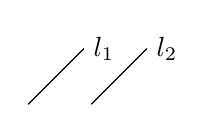
\begin{tikzpicture}
                \draw (0, 0) -- +(45:1) node[right]{$ l_1 $};
                \draw (0.8, 0) -- +(45:1) node[right]{$ l_2 $};
            \end{tikzpicture}
        \end{figure} \\
        Тогда $ b_1 \ne 0 $ и $ \dfrac{b_2}{b_1} = \dfrac{a_2}{a_1} = k $ \\
        В этом случае замена
        $$ u = a_1x + b_1y, \qquad y = \frac1{b_1}(u - a_1x), \qquad y' = \frac1{b_1}(u' - a_1) $$
        сразу приводит уравнение к уравнению с разделяющимися переменными:
        $$ u' = b_1h \bigg( \frac{u + c_1}{ku + c_2} \bigg) + a_1 $$
    \end{itemize}
    \item[\rom8.] Обощённо-однородное уравнение:
    \begin{itemize}
    	\item
        \begin{definition}
            Уравнение называется обощённо-однородным, если каждое его слагаемое имеет один и тот же суммарный порядок по $ x $ и $ y $ при условии, что $ x, \di x $ имеют порядок 1, а $ u, \di y $ -- порядок $ m $
        \end{definition}
        Тогда $ y' = \frac{\di x}{\di y} $ имеет порядок $ m - 1 $ \\
        Аргументы входящих в уравнение функций типа логарифма или тригонометрических должны иметь нулевой порядок \\
        Таким образом, чтобы установить, является ли уравнение обобщённо-однородным, надо приправнять порядки всех слагаемых, получая систему многих уравнений с одной неизвестной $ m $. Если повезёт, такое число $ m $ найдётся. Тогда замена
        $$ y = z^m, \qquad y' = mz^{m - 1}, \qquad z = y^{\faktor1m} $$
        сведёт уравнение к однородному \\
        Проблема возникает, когда замена потребует выполнения условия $ y > 0 $, например, когда $ m = 2 $ или $ m = -\half $. При отсутствии инвариантности относительно замены $ y $ на $ -\vawe{y} $ уравнение придётся решать два раза \\
        Этого можно избежать, сделав более сложную замену:
        \item Бдуем считать, что $ x $ имеет порядок $ \alpha $, а $ y $ имеет порядок $ \beta $ \\
        Тогда $ y' $ имеет порядок $ \beta - \alpha $. Приравнивая суммарные порядки всех слагаемых, находим связь между $ \alpha $ и $ \beta $: $ \beta = k\alpha $ \\
        После этого делается замена $ y^\alpha = ux^\beta $ с выбранным должным образом значением $ \alpha $, в которой наличие новой переменной $ u $ в первой степени позволяет избежать фиксации знаков
    \end{itemize}
\end{enumerate}
